%
\hsection{\crowsFoot{E}{O1}{F}{OM}}%
\label{sec:rm:ef}%
%
\begin{figure}%
\centering%
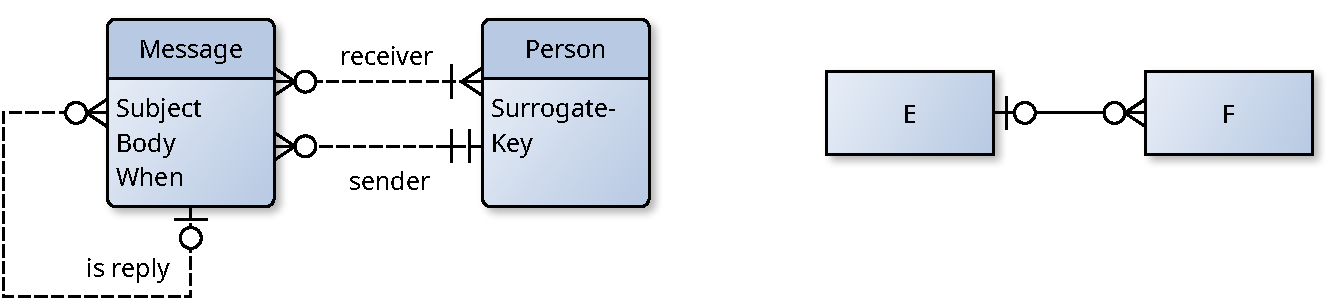
\includegraphics[width=0.9\linewidth]{\currentDir/EF}%
\caption{We encountered the \crowsFoot{E}{O1}{F}{OM} relationship pattern in \cref{fig:erdMessage1}.}%
\label{fig:rm:ef}%
\end{figure}%
%
\gitLoadAndExecSQL{EF_1_tables}{}{conceptualToRelational}{EF_1_tables.sql}{relationships}{}{}%
\listingSQLandOutput{EF_1_tables}{%
The three-table realization of an \crowsFoot{E}{O1}{F}{OM} conceptual relationship.%
}{}%
%
\gitLoadAndExecSQL{EF_1_insert_and_select}{}{conceptualToRelational}{EF_1_insert_and_select.sql}{relationships}{}{}%
\listingSQLandOutput{EF_1_insert_and_select}{%
Inserting into and selecting data from the three-table realization of an \crowsFoot{E}{O1}{F}{OM} conceptual relationship given in \cref{lst:EF_1_tables}.%
}{}%
%
\gitExec{cdtrmTableEO}{\databasesCodeRepo}{conceptualToRelational}{../_scripts_/db_table_to_latex_table.sh relationships e eid;x}%
\gitExec{cdtrmTableFO}{\databasesCodeRepo}{conceptualToRelational}{../_scripts_/db_table_to_latex_table.sh relationships f fid;y}%
\gitExec{cdtrmTableREF}{\databasesCodeRepo}{conceptualToRelational}{../_scripts_/db_table_to_latex_table.sh relationships relate_e_and_f fkeid;fkfid}%
%
\begin{figure}%
\centering%
\floatSep%
\input{\gitFile{cdtrmTableEO}}%
\floatSep%
\input{\gitFile{cdtrmTableFO}}%
\floatSep%
\input{\gitFile{cdtrmTableREF}}%
\floatSep%
\caption{The contents of the the tables in the three-table implementation of the \crowsFoot{E}{O1}{B}{OM} conceptual relationship after executing \cref{lst:EF_1_insert_and_select}.}%
\label{fig:rm:ef:1:tables}%
\end{figure}%
%
\gitLoadAndExecSQL{EF_cleanup}{}{conceptualToRelational}{EF_cleanup.sql}{relationships}{}{}%
\listingSQLandOutput{EF_cleanup}{%
Deleting the tables created in \cref{lst:EF_1_tables}.}{}%
%
\gitLoadAndExecSQL{EF_2_tables}{}{conceptualToRelational}{EF_2_tables.sql}{relationships}{}{}%
\listingSQLandOutput{EF_2_tables}{%
A two-table realization of an \crowsFoot{E}{O1}{F}{M1} conceptual relationship.%
}{}%
%
\gitLoadAndExecSQL{EF_2_insert_and_select}{}{conceptualToRelational}{EF_2_insert_and_select.sql}{relationships}{}{}%
\listingSQLandOutput{EF_2_insert_and_select}{%
Inserting into and selecting data from the two-table realization of an \crowsFoot{E}{O1}{F}{OM} conceptual relationship given in \cref{lst:EF_2_tables}.%
}{}%
%
\gitExec{cdtrmTableET}{\databasesCodeRepo}{conceptualToRelational}{../_scripts_/db_table_to_latex_table.sh relationships e eid;x}%
\gitExec{cdtrmTableFT}{\databasesCodeRepo}{conceptualToRelational}{../_scripts_/db_table_to_latex_table.sh relationships f fid;fkeid;y}%
%
\begin{figure}%
\centering%
\floatSep%
\input{\gitFile{cdtrmTableET}}%
\floatSep%
\input{\gitFile{cdtrmTableFT}}%
\floatSep%
\caption{The contents of the the tables in the two-table implementation of the \crowsFoot{E}{O1}{B}{OM} conceptual relationship after executing \cref{lst:EF_2_insert_and_select}.}%
\label{fig:rm:ef:2:tables}%
\end{figure}%
%
We have the two entity types~E and~F.
Each entity of type~E may be connected to zero, one, or multiple entities of type~F.
Each entity of type~F is connected to zero or one entity of type~E.

We encountered this relationship pattern back in \cref{fig:erdMessage1}, where we tried to model the messaging subsystem for our teaching management platform.
A message can either be a new message or a reply to exactly one existing message.
There may be zero, one, or many replies to any existing message.
This situation is sketched in \cref{fig:rm:ef}.

We need a table~\sqlil{e} for the entities of type~E and a table~\sqlil{f} for the entities of type~F.
Both have their respective surrogate primary keys~\sqlil{eid} and~\sqlil{fid} and we also add the example attributes~\sqlil{x} and~\sqlil{y} to them, respectively.
Apart from that, there can again be two solutions to implementing this relationship:
We can use three tables or two, again, depending on how many entities of types~E and~F are actually related.

We may use a third table~\sqlil{relate_e_and_f} relating the entities of type~E to those of type~F.
This approach is illustrated in \cref{lst:EF_1_tables}.
There will be two columns in that table.
The first one, \sqlil{fkeid}, holds the reference to the primary key~\sqlil{eid} of the E~entities.
The second one, \sqlil{fkfid}, holds the reference to the primary key~\sqlil{fid} of the F~entities.
Since we only store the pairs that exist, both columns are~\sqlil{NOT NULL} and have~\sqlil{REFERENCES} constraints to their respective foreign keys.

Since each entity of type~F can only be connected to at most one entity of type~E, there will be a~\sqlil{UNIQUE} constraint on the column~\sqlil{fkfid} and it would be the primary key of table~\sqlil{relate_e_and_f}.
It needs to be the primary key because the values in column~\sqlil{fkeid} do not need to be unique -- one entity of type~E can be related to many entities of type~F.

In \cref{lst:EF_1_insert_and_select}, we insert some data into the tables.
Since both relationship ends are optional, we can first populate tables~\sqlil{e} and~\sqlil{f}.
Then we can establish the relationships by adding rows to table~\sqlil{relate_e_and_f}.
The contents of the three tables after executing \cref{lst:EF_1_insert_and_select} are given in \cref{fig:rm:ef:1:tables}.%
%
\begin{sloppypar}%
This is the recommended solution in~\cite{S2024D:MEDTRDM}, but we face a similar situation as back in~\dref{sec:rm:ab}:
It is efficient only if there are not too many E\nobreakdashes-F pairs that are related.
If almost all entities of type~F are related to one entity of type~E, then the table~\sqlil{relate_e_and_f} is about as same as big as the table~F.
Instead of simply storing the keys of the related E~entities in the table~\sqlil{f}, we now have another table that stores these keys \emph{and} the primary keys of the \sqlil{f}~table.
Also, we would again need two \sqlil{INNER JOIN} statements instead of one when we merge the data, as shown in \cref{lst:EF_1_insert_and_select}.%
\end{sloppypar}%
%
The two-table solution is illustrated in \cref{lst:EF_2_tables}.
Here, we need to add a foreign key column~\sqlil{fkeid} to the table~\sqlil{f}.
This column has a \sqlil{REFERENCES} constraint pointing to column~\sqlil{eid} of table~\sqlil{e}.
The value of this column can be \sqlil{NULL}, because not all rows in~\sqlil{f} need to be related to rows in~\sqlil{e}.
Different from the \crowsFoot{A}{O1}{B}{O1} situation in~\cref{lst:AB_2_tables}, there also \emph{should not} be a \sqlil{UNIQUE} constraint here, because each row of~\sqlil{E} can be related to multiple rows in~\sqlil{f}.

We store some data into the three tables in \cref{lst:EF_2_insert_and_select}.
We can do this by first inserting rows into table~\sqlil{e}.
Then we add rows to table~\sqlil{f}.
For each such row, we can provide a valid foreign key~\sqlil{fkeid} to a row in table~\sqlil{e} identified by primary key~\sqlil{eid}.
This means that the new row in table~\sqlil{f} will be related to the existing row in table~\sqlil{e}.
We can also store~\sqlil{NULL} as \sqlil{fkeid}, in which case the row in table~\sqlil{f} is not related to any row in table~\sqlil{e}.
The contents of the two tables after executing \cref{lst:EF_2_insert_and_select} are given in \cref{fig:rm:ef:2:tables}.
We also only need a single \sqlil{INNER JOIN} to merge the data, as illustrated in \cref{lst:EF_2_insert_and_select}.

This solution has another useful aspect:
In the three-table solution, I can create an \sqlil{INSERT} or \sqlil{UPDATE} query to \sqlil{relate_e_and_f} that fails, namely if I try to relate a row of~\sqlil{f} to more than one row in~\sqlil{e}.
This is not possible in the two-table solution, because each row of~\sqlil{f} only has one attribute value~\sqlil{fkeid}.%
%
\FloatBarrier%
\endhsection%
%
